To assess the size of opportunity for our aforementioned optimizations to reduce interactive latency in computational notebooks, we evaluate two real world notebook corpora.

One corpus is collected from students in the \textbf{Data 100} class offered at UC Berkeley. Data 100 is an intermediate data science course offered at the undergraduate level, covering topics on tools and methods for data analysis and machine learning.  This corpus contains 210 notebooks across four different assignments, complete with the \emph{history} of cell execution content and completion times captured by instrumenting a custom Jupyter extension.

We also collected Jupyter notebooks from \textbf{Github} comprising a more diverse group of users than Data 100.  Jupyter’s IPython kernel stores the code corresponding to each individual cell executions in a local \code{history.sqlite} file\footnote{\url{https://ipython.readthedocs.io/en/stable/api/generated/IPython.core.history.html}}.  We used 429 notebook execution histories that Macke et al.~\cite{mackefine} scraped from Github that also contained pandas operations. 

To assess optimization opportunities, we first quantify \thinktime between cell executions, and then evaluate the prevalence of the code patterns discussed in Section~\ref{sec:tasks}.

\subsection{Think-Time Opportunities}
\label{sec:thinktime}
Our proposed opportunistic evaluation framework takes advantage of user \thinktime to asynchronously process non-critical operators to reduce the latency of future interactions.
To quantify \thinktime, we measure the time lapsed between the completion of a cell execution and the start of the next cell execution using the timestamps in the cell execution and completion records, as collected by our Jupyter notebook extension.
Note that the \thinktime statistics are collected only on the Data 100 corpus, as the timestamp information is not available in the Github corpus.
Figure~\ref{fig:think} shows the distribution of \thinktime intervals on the left, measured in seconds, between consecutive cell executions across all notebooks, while the right part of Figure~\ref{fig:think} shows the distribution of the median \thinktime intervals, measured in seconds, within each notebook.  
We removed automatic cell re-execution (``run all'') from the dataset.
We can see that while there are many cells that were executed quickly, there exist cells that had ample \thinktime---the 75th percentile \thinktime is 23 seconds. 

\begin{figure}[h!]
     \centering
     \begin{subfigure}%[b]{0.4\textwidth}
         \centering
         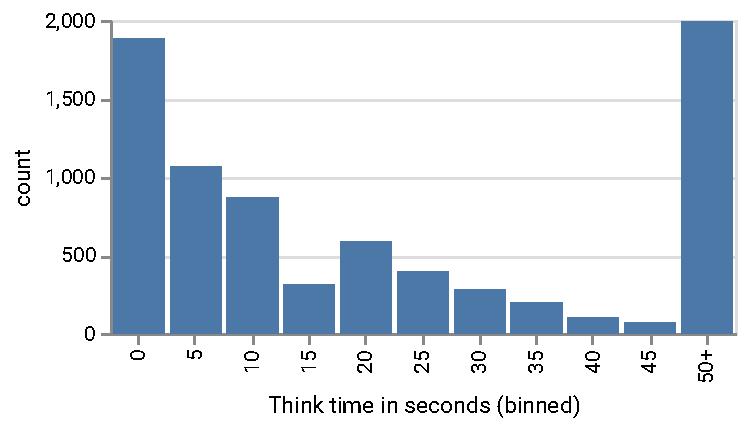
\includegraphics[width=0.4\textwidth]{submissions/interactivity/figures/ds_think_cell_v2.pdf}
         %\caption{\Thinktime between cell executions.}
         %\label{fig:think_cell}
     \end{subfigure}
    \hfill
     \begin{subfigure}%[b]{0.4\textwidth}
         \centering
         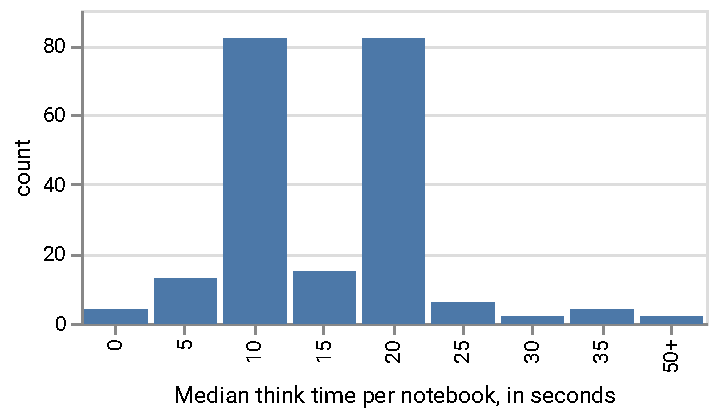
\includegraphics[width=0.4\textwidth]{submissions/interactivity/figures/ds_think_nb_v2.pdf}
         %\caption{Median \thinktime per notebook across cells.}
         %\label{fig:think_nb}
     \end{subfigure}
        \caption{\Thinktime the average ``\thinktime'' between cell executions and the average \thinktime per notebook. (left) \Thinktime between cell executions; (right) Median \thinktime per notebook across cells.}
        \label{fig:think}
\end{figure}


\subsection{Program Transformation Opportunities}

\topic{Interaction-Based Reordering} To assess the opportunities to apply operator reordering to prioritize interactions, we evaluate the number of non-critical operators specified before each interaction.  We use the operator DAG, to be described in Section~\ref{sec:dag}, to determine the dependencies of an interaction and count the number of operators that are not dependencies, i.e., non-critical operators, specified above the interaction.
Figure~\ref{fig:nooo} shows the distributions for the two datasets.
In both cases, non-critical operators present a major opportunity: the Data 100 and Github corpus have, respectively, 54\% and 42\% interactions with non-critical operators.


\begin{figure}[h!]
     \centering
    \begin{subfigure}%[b]{0.4\textwidth}
         \centering
         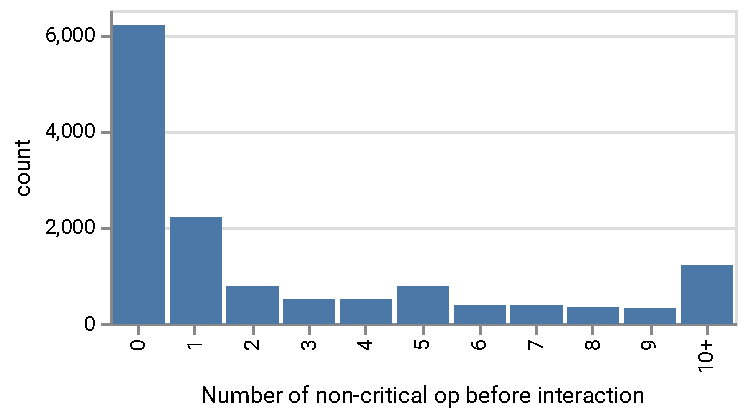
\includegraphics[width=0.4\textwidth]{submissions/interactivity/figures/ds_nooo_v2.pdf}
         %\caption{Data 100: $\mu$ = 4, $\sigma$ = 5}
         %\label{fig:ds_nooo}
     \end{subfigure}
     \hfill
     \begin{subfigure}%[b]{0.4\textwidth}
         \centering
         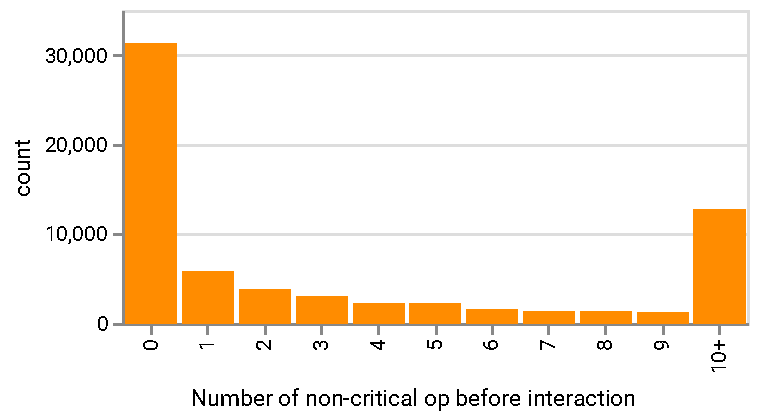
\includegraphics[width=0.4\textwidth]{submissions/interactivity/figures/gb_nooo_v2.pdf}
         %\caption{Github: $\mu$ = 7, $\sigma$ = 11}
         %\label{fig:gh_nooo}
     \end{subfigure}
     \caption{Number of non-critical operators before interactions. (left) Data 100: $\mu$ = 4, $\sigma$ = 5; (right) Github: $\mu$ = 7, $\sigma$ = 11}
    \label{fig:nooo}
\end{figure}

\begin{figure}[h!]
     \centering
     \begin{subfigure}%[b]{0.4\textwidth}
         \centering
         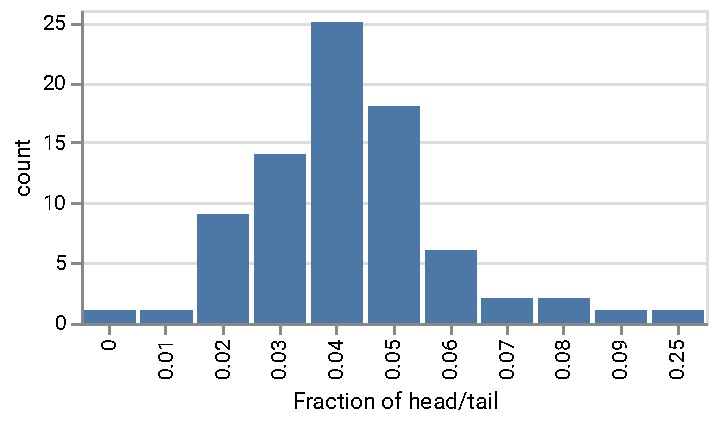
\includegraphics[width=0.4\textwidth]{submissions/interactivity/figures/ds_nht_v2.pdf}
         %\caption{Data 100: $\mu$ = 0.04, $\sigma$ = 0.028}
         %\label{fig:ds_nht}
     \end{subfigure}
     \hfill
     \begin{subfigure}%[b]{0.4\textwidth}
         \centering
         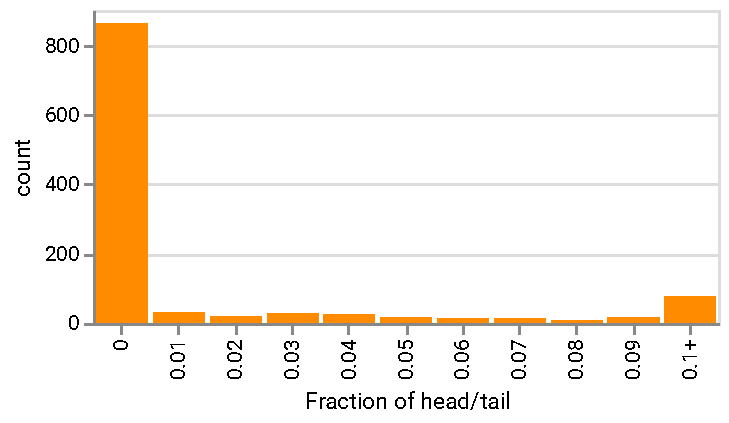
\includegraphics[width=0.4\textwidth]{submissions/interactivity/figures/gb_nht_v2.pdf}
         %\caption{Github: $\mu$ = 0.11, $\sigma$ = 0.21}
         %\label{fig:gh_nht}
     \end{subfigure}
     \caption{Stats for head/tail interactions used in each notebook. (left) Data 100: $\mu$ = 0.04, $\sigma$ = 0.028; (right) Github: $\mu$ = 0.11, $\sigma$ = 0.21}
     \label{fig:stats}
\end{figure}

\begin{figure}[h!]
     \centering
     \begin{subfigure}%[b]{0.4\textwidth}
         \centering
         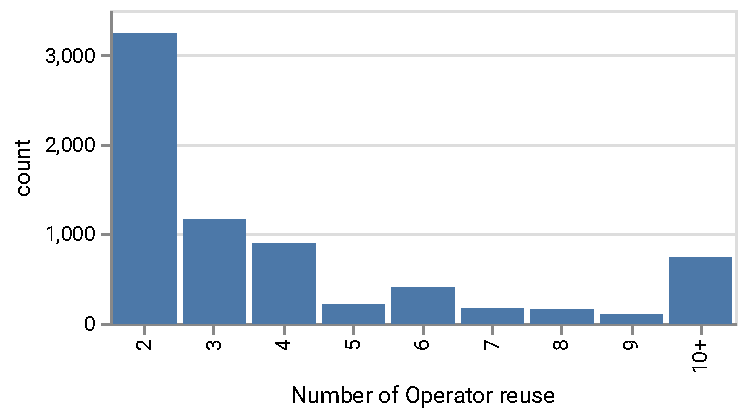
\includegraphics[width=0.4\textwidth]{submissions/interactivity/figures/ds_nre_v2.pdf}
         %\caption{Data 100: $\mu$ = 5, $\eta$ = 3, $\sigma$ = 8}
         %\label{fig:ds_nre}
     \end{subfigure}
     \hfill
     \begin{subfigure}%[b]{0.4\textwidth}
         \centering
         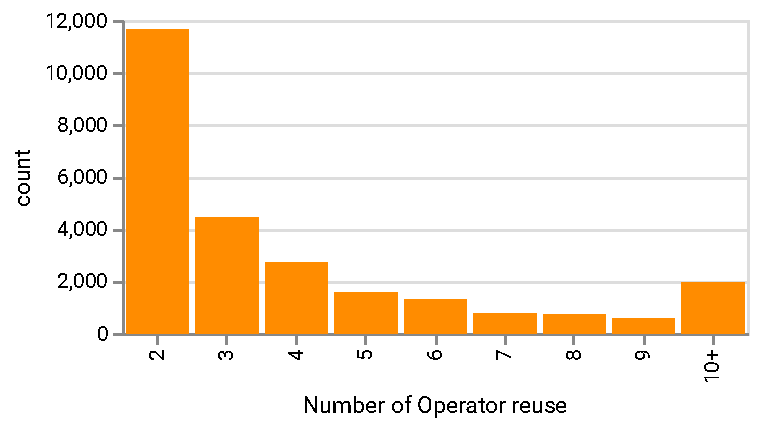
\includegraphics[width=0.4\textwidth]{submissions/interactivity/figures/gb_nre_v2.pdf}
        %  \vspace{-15pt}
         %\caption{Github: $\mu$ = 7, $\eta$ = 3, $\sigma$ = 14}
         %\label{fig:gh_nre}
     \end{subfigure}
    \caption{Distribution of number of operators that can benefit from reuse. (left) Data 100: $\mu$ = 5, $\eta$ = 3, $\sigma$ = 8; (right) Github: $\mu$ = 7, $\eta$ = 3, $\sigma$ = 14}
    \label{fig:reuse}
\end{figure}


\topic{Prioritizing Partial Results}  The optimization for prioritizing partial results via predicate pushdown can be applied effectively to many cases when predicates are involved in queries with multiple operators.  The most common predicates in the dataframe setting are \code{head()} and \code{tail()}, which show the top and bottom $K$ rows of the dataframe, respectively. 
Figure~\ref{fig:stats} show the distribution of the fraction of interactions that are either \code{head} or \code{tail} in each notebook. 
We see that partial results views are much more common in the GitHub dataset than Data 100. This could be due to the fact that users on GitHub tend to keep the cell output area short for better rendering of the notebook by Github, but further studies are needed to corroborate this hypothesis. Lastly, partial views are not nearly as prevalent as non-critical operators before an interaction, accounting only for $<20\%$ of the interactions. 

\topic{Reuse of Intermediate Results} 
Since dataframe queries are incrementally constructed, with subsequent queries building on top of previous ones, another common query optimization technique that is applicable is caching these intermediate results.
To assess the opportunities to speed up queries by caching, we evaluate the number of times an operator is shared by different interactions but not stored as a variable by the user.
Ideally, we would also have the execution times of the individual operators, which is not possible without a full replay.  We present an initial analysis that only assesses the \emph{existence} of reuse opportunities, as shown
in Figure~\ref{fig:reuse}. Both the Data 100 and Github datasets have a median of 3 operators that can benefit from reuse.


\vspace{2pt}
\noindent Of the types of optimizations explored, operator reordering appears to be the most common.
Thus, we focus our initial explorations of opportunistic evaluation on operator reordering for asynchronous execution during \thinktime, while supporting preemption to interrupt asynchronous execution and prioritize interaction.
